% ----------------------------------------------------------------------------------------------------------
% Anhang
% ----------------------------------------------------------------------------------------------------------
\pagenumbering{Roman}
\setcounter{page}{1}
\lhead{Anhang \thesection}

\begin{appendix}
\section*{Anhang}
\phantomsection
\addcontentsline{toc}{section}{Anhang}
\addtocontents{toc}{\vspace{-0.5em}}

\vspace{1em}
\begin{minipage}{\linewidth}
	\centering
	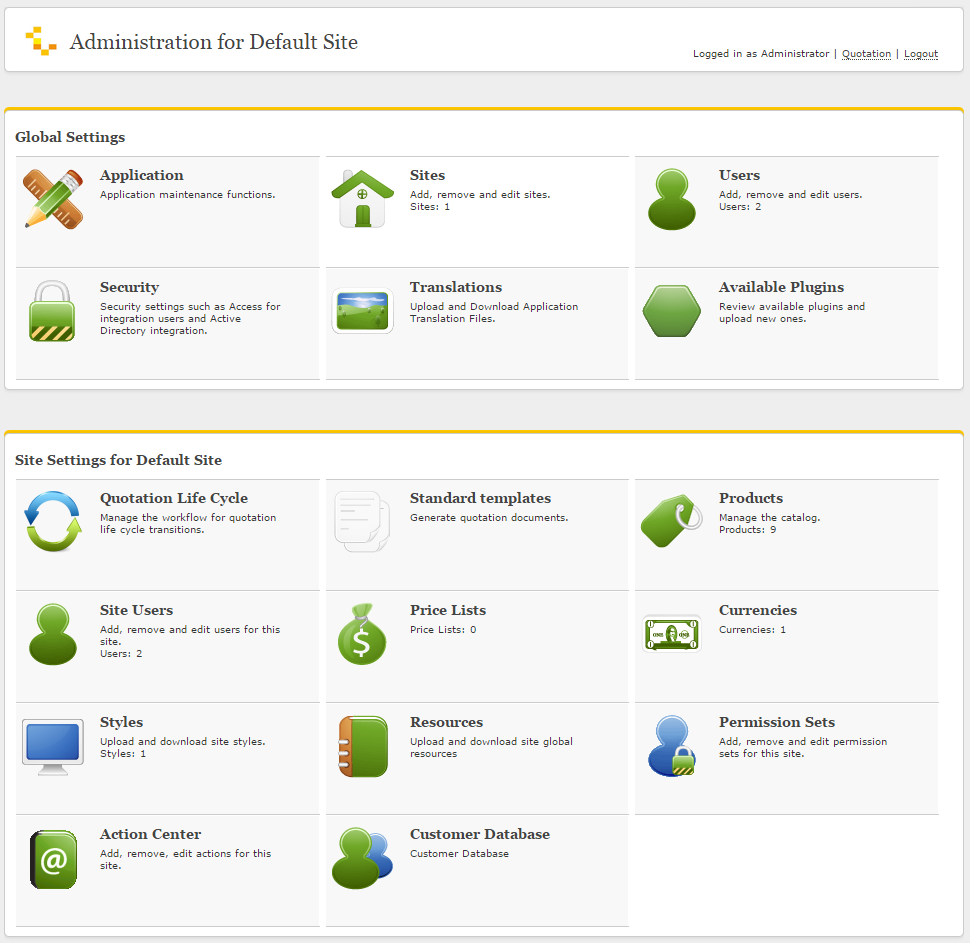
\includegraphics[width=1\linewidth]{Abbildungen/tcsiteAdministration.PNG}
	\captionof{figure}[tcsiteAdministration]{TCsite Administrationsoberfläche}
	\label{app:tcsiteAdministration}
\end{minipage}
\vspace{1em}

\vspace{1em}
\begin{minipage}{\linewidth}
	\centering
	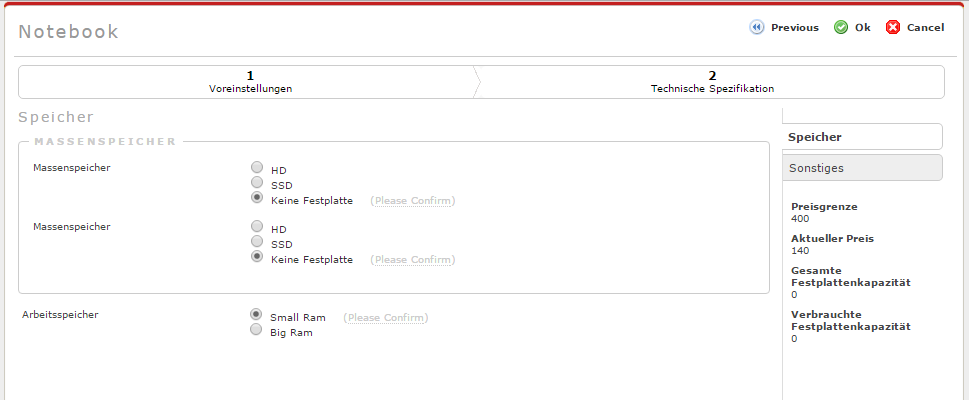
\includegraphics[width=1\linewidth]{Abbildungen/tcSiteConfigurationOptionalGroups.PNG}
	\captionof{figure}[tcSiteConfigurationOptionalGroups]{Darstellung optionaler Groups in TCsite}
	\label{app:tcSiteConfigurationOptionalGroups}
\end{minipage}
\vspace{1em}

\vspace{1em}
\begin{minipage}{\linewidth}
	\centering
	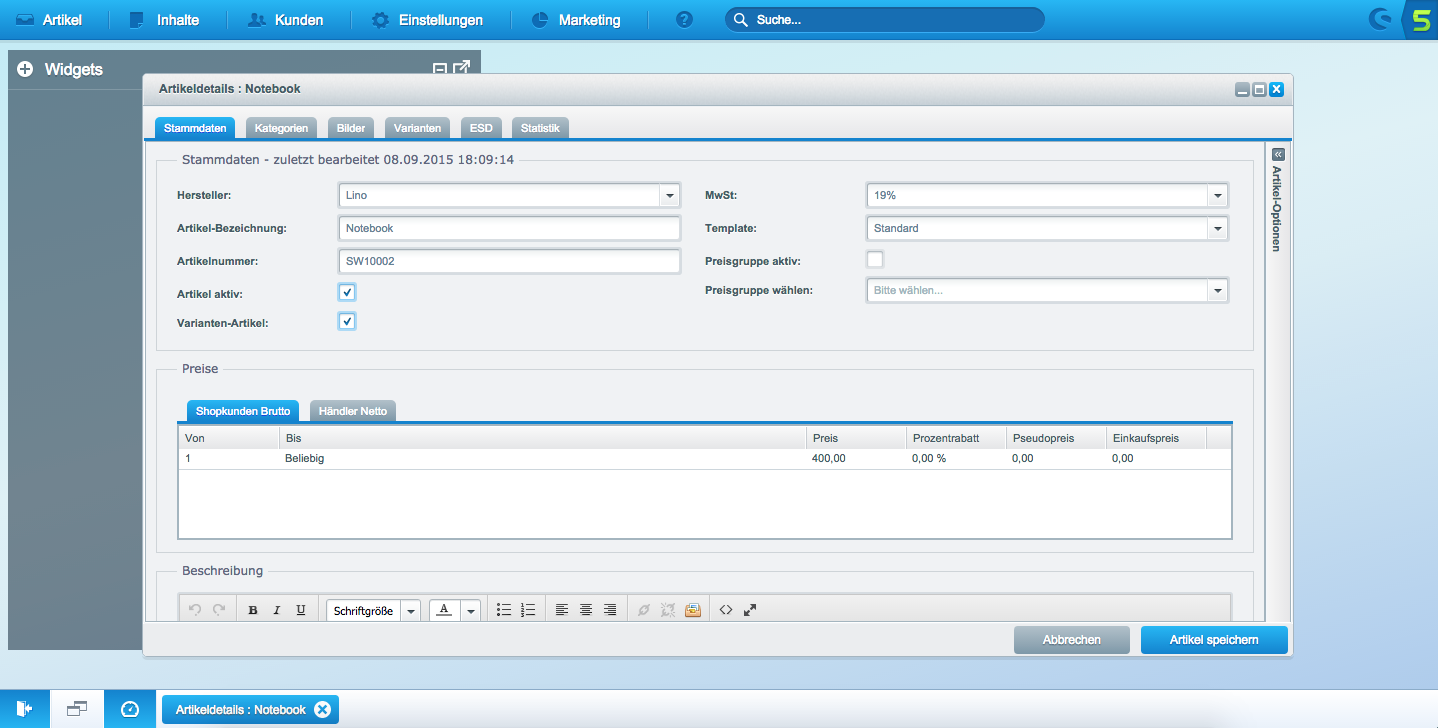
\includegraphics[width=1\linewidth]{Abbildungen/shopwareBackendArtikel.png}
	\captionof{figure}[shopwareBackendArtikel]{Anlegen eines Artikels im Backend}
	\label{app:shopwareBackendArtikel}
\end{minipage}
\vspace{1em}

\vspace{1em}
\begin{minipage}{\linewidth}
	\centering
	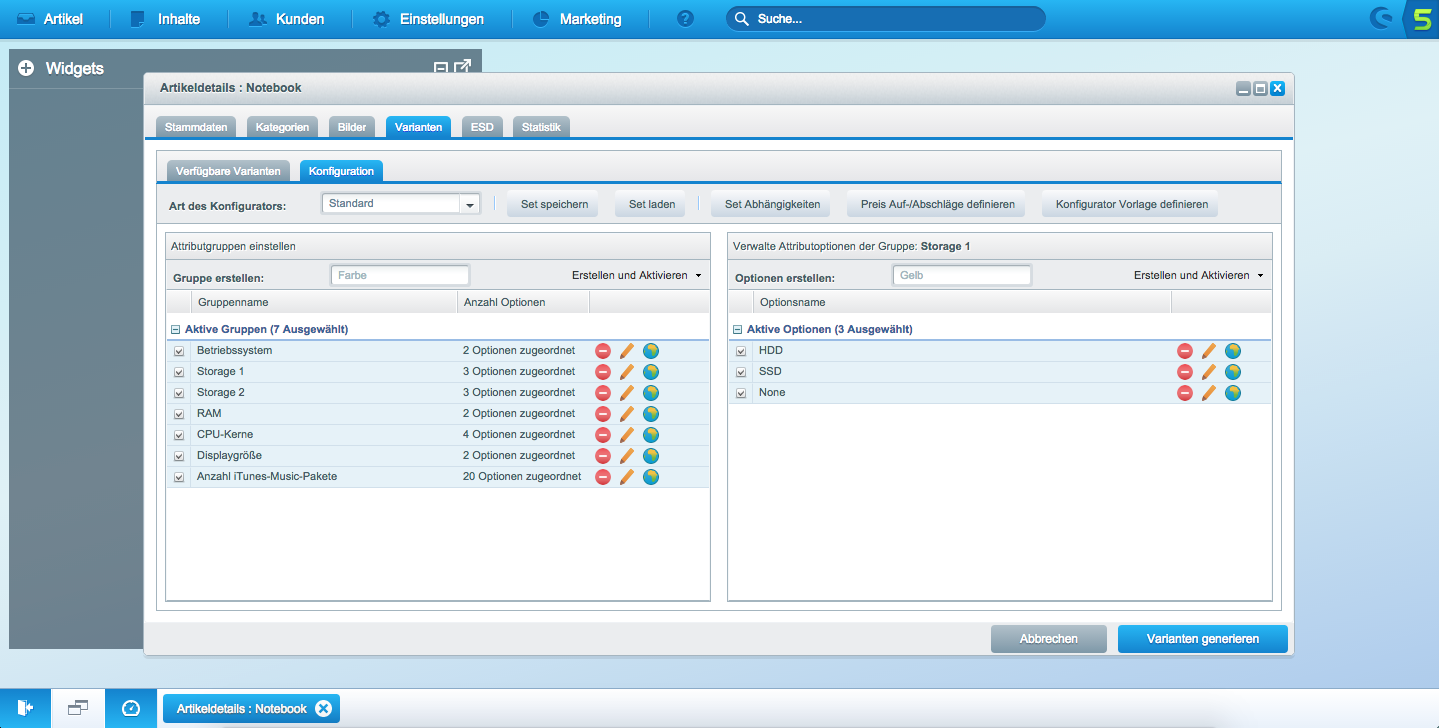
\includegraphics[width=1\linewidth]{Abbildungen/shopwareBackendArtikelVarianten.png}
	\captionof{figure}[shopwareBackendArtikelVarianten]{Generieren der Varianten im Backend}
	\label{app:shopwareBackendArtikelVarianten}
\end{minipage}
\vspace{1em}

\vspace{1em}
\begin{minipage}{\linewidth}
	\centering
	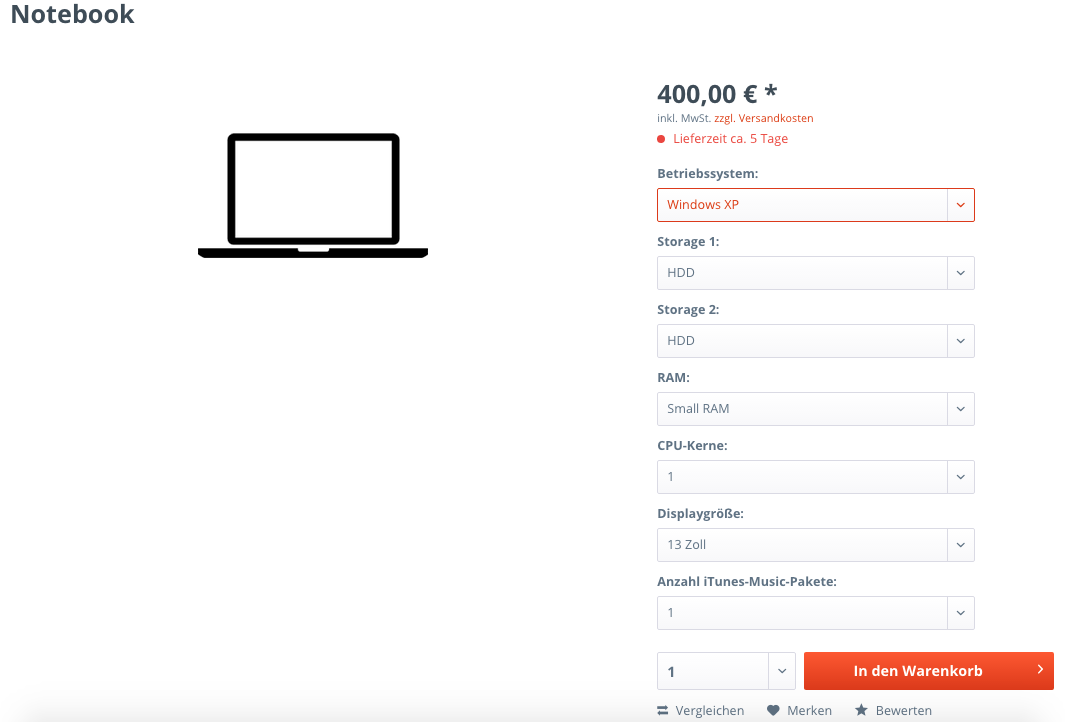
\includegraphics[width=1\linewidth]{Abbildungen/shopwareNotebookDetail.png}
	\captionof{figure}[shopwareNotebookDetail]{Detailansicht eines konfigurierbaren Notebooks in shopware.}
	\label{app:shopwareNotebookDetail}
\end{minipage}
\vspace{1em}

\vspace{1em}
\begin{minipage}{\linewidth}
	\centering
	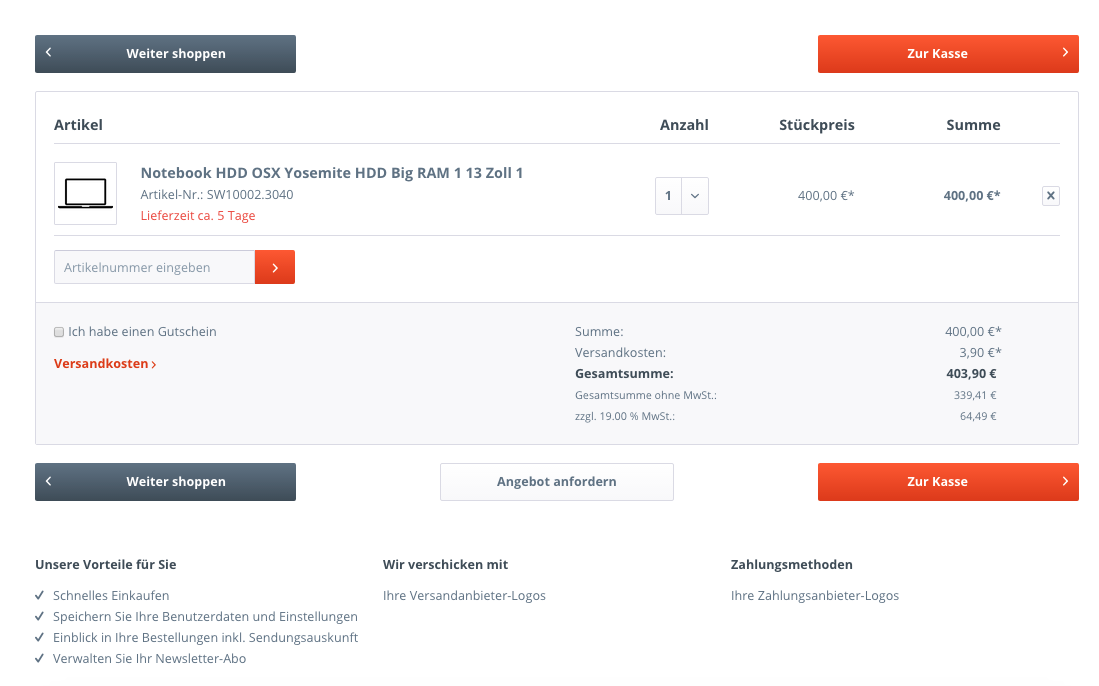
\includegraphics[width=1\linewidth]{Abbildungen/shopwareNotebookWarenkorb.png}
	\captionof{figure}[shopwareNotebookWarenkorb]{Warenkorb mit konfiguriertem Artikel.}
	\label{app:shopwareNotebookWarenkorb}
\end{minipage}
\vspace{1em}

\end{appendix}